\documentclass[
  a4paper,
  spanish,
  12pt,
]{scrartcl}

\linespread{1.05}
%\setlength{\parindent}{18pt}


%-------------------------------------------------------------------------------
%	PAQUETES
%-------------------------------------------------------------------------------

% Idioma

\usepackage{indentfirst}
% Matemáticas

\usepackage{mathrsfs}

\usepackage{config}
\usepackage{amsmath, amsthm, amssymb}
% \usepackage{mathtools}
% \usepackage{commath}
% \usepackage{xfrac}
\usepackage{graphicx}

\newcommand{\norm}[1]{\left \lVert #1 \right \rVert}

% Fuentes personalizadas para utilizar con XeLaTeX o LuaLaTeX

\usepackage[no-math]{fontspec}
\setmainfont[WordSpace=1.3, RawFeature={+ss06}]{EBGaramond}
\setsansfont[Scale=0.9]{Alegreya Sans}
\setmonofont[Scale=0.75]{Bitstream Vera Sans Mono}

\usepackage[math-style=TeX]{unicode-math}
\setmathfont{Garamond Math}[StylisticSet={3}]


% Configuración de microtype

\defaultfontfeatures{Ligatures=TeX,Numbers=Lining}
\usepackage[activate={true,nocompatibility},final,tracking=true,factor=1100,stretch=10,shrink=10]{microtype}
\SetTracking{encoding={*}, shape=sc}{0}

% Enlaces y colores

\usepackage{hyperref}
\usepackage{xcolor}
\hypersetup{
  colorlinks=true,
  citecolor=,
  linkcolor=,
  urlcolor=blue,
}

% Otros elementos de página

\usepackage{enumitem}
\setlist[enumerate]{leftmargin=-\itemindent, itemsep=0pt}
\setlist[itemize]{leftmargin=-\itemindent, itemsep=0pt}
%\setlist[itemize]{leftmargin=*}
%\setlist[enumerate]{leftmargin=*}

\usepackage[labelfont={sc, sf}, textfont=sf]{caption}

\usepackage{booktabs}
\renewcommand\arraystretch{1.5}

% Tikz

\usepackage{tikz}
\usetikzlibrary{babel}
\usepackage{float}

% Código

\usepackage{listings}
\lstset{
	basicstyle=\ttfamily,%
	breaklines=true,%
	captionpos=b,                    % sets the caption-position to bottom
  tabsize=2,	                   % sets default tabsize to 2 spaces
  frame=lines,
  numbers=left,
  stepnumber=1,
  aboveskip=12pt,
  showstringspaces=false,
  keywordstyle=\bfseries,
  commentstyle=\itshape,
  columns=flexible,
}
\renewcommand{\lstlistingname}{Listado}

% ENTORNOS

\usepackage[theorems, skins, breakable]{tcolorbox}

\tcolorboxenvironment{nth}{
	blanker,
	breakable,
	left=12pt,
	before skip=12pt,
	after skip=12pt,
	borderline west={2pt}{0pt}{500},
	before upper={\parindent 12pt},
}

\tcolorboxenvironment{nprop}{
	blanker,
	breakable,
	left=12pt,
	before skip=12pt,
	after skip=12pt,
	borderline west={2pt}{0pt}{42},
	before upper={\parindent 12pt},
}

\tcolorboxenvironment{ncor}{
	blanker,
	breakable,
	left=12pt,
	before skip=12pt,
	after skip=12pt,
	borderline west={2pt}{0pt}{300},
	before upper={\parindent 12pt},
}

\tcolorboxenvironment{ndef}{
	skin=enhancedmiddle jigsaw,
	frame hidden,
	colback= 36,
	breakable = true,
	break at = -6pt,
	top = 4pt,       % Estos márgenes están un poco a ojo
	bottom = 4pt,
	left= 8pt,
	right = 8pt,
	before skip=8pt, % Normalmente dejamos 12pt, pero
	after skip=8pt,  % aquí tenemos espacio adicional por el fondo
	no borderline,
	borderline west={2pt}{0pt}{42},
	before upper={\parindent 12pt},
}

\tcolorboxenvironment{ejer}{
	skin=enhancedmiddle jigsaw,
	frame hidden,
	colback=50,
	breakable = true,
	break at = -6pt,
	top = 4pt,       % Estos márgenes están un poco a ojo
	bottom = 4pt,
	left= 8pt,
	right = 8pt,
	before skip=8pt, % Normalmente dejamos 12pt, pero
	after skip=8pt,  % aquí tenemos espacio adicional por el fondo
	no borderline,
	borderline west={2pt}{0pt}{500},
	borderline east={2pt}{0pt}{50},
	before upper={\parindent 12pt},
}


% Márgenes
\usepackage[bottom=3.125cm, top=2.5cm, left=3.5cm, right=3.5cm, marginparwidth=70pt]{geometry}

%dealing with (sub/subsub)sections
%\let\raggedsection\centering%Center all sectioningheads
%all levels have something in common, let's save typing:
\RedeclareSectionCommands[beforeskip=-3ex,
afterskip=2ex]{section,subsection,subsubsection}
\addtokomafont{section}{\normalfont\large\textsc}
\RedeclareSectionCommand[beforeskip=-6ex]{section}
\addtokomafont{subsection}{\normalfont\itshape}

%-------------------------------------------------------------------------------
%	CONTENIDO
%-------------------------------------------------------------------------------

\begin{document}

\begin{flushright}
  Ricardo Ruiz Fernández de Alba\vspace{.5em}

  \textit{Topología II}

  Doble Grado en Ingeniería Informática y Matemáticas

  \textsc{Universidad de Granada}\vspace{.5em}

  \today\vspace{.5em}
\end{flushright}

\begin{flushleft}
  \scshape\Large Relación de Ejercicios del Tema 2
\end{flushleft}

Todos los espacios topológicos considerados en esta relación de ejercicios se suponen conexos y localmente arcoconexos, luego arcoconexos.\\

\begin{ejer}
(1) Dados dos aplicaciones recubridoras $\pi_{i}: \tilde{X}_{i} \rightarrow X_{i}, i=1,2$, demuestra que $\pi_{1} \times \pi_{2}: \tilde{X}_{1} \times \tilde{X}_{2} \rightarrow$ $X_{1} \times X_{2}$ es también aplicación recubridora.\\
\end{ejer}

\begin{sol}
Si $\pi_1, \pi_2$ son continuas, entonces $\pi_1 \times \pi_2$ lo es.
Si $\pi_1, \pi_2$ son sobreyectivas, entonces $\pi_1 \times \pi_2$ lo es. Ya que:

$$
(\pi_1 \times \pi_2)(\tilde{X_1} \times \tilde{X_2}) = \pi_1(\tilde{X_1}) \times \pi_1(\tilde{X_2}) = X_1 \times X_2
$$

Por tanto $\pi_1 \times \pi_2$ es continua y sobreyectiva.

Sea $(x_1, x_2) \in X_1 \times X_2$, entonces $x_1 \in X_1$ y $x_2 \in X_2$.
Por ser $\pi_1$ aplicación recubridora, existirá $U_1 \in \mathcal{U}^{x_1}$ entorno de $x_1$ tal que
$\pi_1^{-1}(U_1) = \bigsqcup_{i \in \Lambda} V_i$ con $V_i \cong U_1 \quad \forall i \in \Lambda$ mediante
el homeomorfismo $\varphi_i$.

Por ser $\pi_2$ aplicación recubridora, existirá $U_2 \in \mathcal{U}^{x_2}$ entorno de $x_2$ tal que
$\pi_2^{-1}(U_2) = \bigsqcup_{i \in \Lambda} \tilde{V}_i$ con $\tilde{V}_i \cong U_2 \quad \forall i \in \Lambda$ mediante
el homeomorfismo $\tilde{\varphi}_i$

Sea ahora $W = U_1 \times U_2$, es claramente un entorno de $(x_1, x_2)$. Es decir, $W \in \mathcal{U}^{(x_1, x_2)}$.
Además,

$$
(\pi_1 \times \pi_2)^{-1}(W) = \pi_1^{-1}(U_1) \times \pi_2^{-1}(U_2) = 
\left(\bigsqcup_{i \in \Lambda} V_i \right)  \times \left(\bigsqcup_{i \in \Lambda} \tilde{V}_i \right) 
= \bigsqcup_{i \in \Lambda} (V_i \times \tilde{V}_i )
$$

donde $V_i \times \tilde{V}_i \cong U_1 \times U_2$ dado por el homeomorfismo $\Phi_i = \varphi_i \times \tilde{\varphi}_i$.

Por tanto $\pi_1 \times \pi_2$ es aplicación recubridora.
\end{sol}

\begin{ejer}
(2) Consideremos el espacio recubridor $(\mathbb{R}, \rho)$ de $\mathbb{S}^{1}$ donde $\rho(t)=e^{2 \pi t i}$ para todo $t \in \mathbb{R}$. Demostrar que la aplicación $\left.\rho\right|_{(0,2)}:(0,2) \rightarrow \mathbb{S}^{1}$ es continua, abierta y sobreyectiva pero no es recubridora. ¿Existe alguna aplicación $\psi:(0,2) \rightarrow \mathbb{S}^{1}$ tal que $((0,2), \psi)$ sea un recubridor de $\mathbb{S}^{1}$ ?\\
\end{ejer}

\begin{sol}
Necesariamente no se debe cumplir la tercera propiedad de la definición de aplicación recubridora.
En efecto, sea $1 \in \mathbb{S}^1$ y sea $U$ un arco de circunferencia abierto, entorno suyo. Entonces,

$$
\rho\vert_{\;]0,2[\;} (U) = \;]0, \varepsilon[\; \cup \;]1-\varepsilon, 1+\varepsilon[\; \cup \;]2-\varepsilon, 2[\;
$$
y 
$$
\rho\vert_{\;]0, \varepsilon[\;} \to U
$$

no es un homeomorfismo porque no es sobreyectiva (el \( 1 \) no es imagen de ningún elemento del dominio).

\end{sol}

\newpage

\begin{ejer}
(3) Sean $X$ un espacio topológico, $(\widetilde{X}, \pi)$ un recubridor de $X$ y $(\widetilde{\widetilde{X}}, \psi)$ un recubridor de $\widetilde{X}$. Demostrar que si el recubridor $(\widetilde{X}, \pi)$ es finito, entonces $(\widetilde{\widetilde{X}}, \pi \circ \psi)$ es un recubridor de $X$.\\
\end{ejer}

\begin{figure}[h]
    \centering
    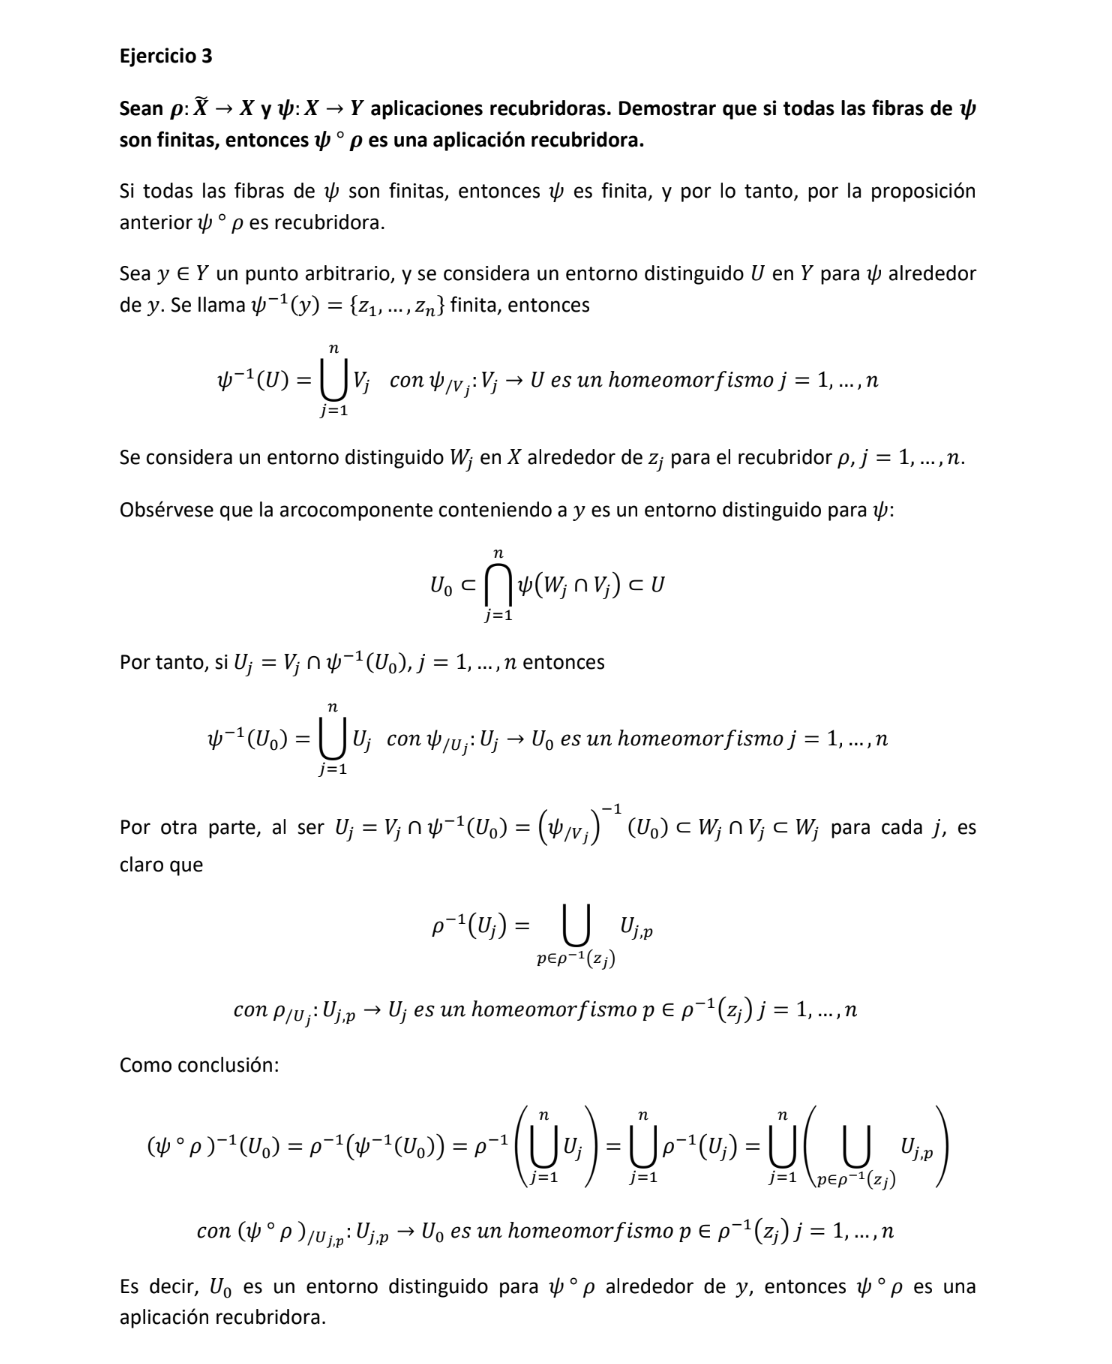
\includegraphics[width=\textwidth]{ej3.png}
    \label{fig:etiqueta}
\end{figure}

\newpage

\begin{ejer}
(4) Sean $X=\left\{(x, y, z) \in \mathbb{R}^{3}: x^{2}+y^{2}-z^{2}=1\right\}$ y $\widetilde{X}=\left\{(x, y, z) \in \mathbb{R}^{3}: z=x^{2}+y^{2}\right\}$. Construir explícitamente una aplicación recubridora $\pi: \widetilde{X} \rightarrow X$. ¿Existe una aplicación recubridora $\psi$ : $X \rightarrow \widetilde{X}$ ?\\
\end{ejer}

\begin{ejer}
(5) Calcular el recubridor universal del toro $T=\mathbb{S}^{1} \times \mathbb{S}^{1}$ y del cilindro $C=\mathbb{S}^{1} \times \mathbb{R}$.\\
\end{ejer}

\begin{ejer}
(6) Construir una aplicación recubridora de dos hojas $\pi: T \rightarrow K$, donde $T$ es el toro y $K$ es la botella de Klein. Deducir que $\mathbb{R}^{2}$ es el recubridor universal de $K$.\\
\end{ejer}

\begin{ejer}
(7) Construir una aplicación recubridora de dos hojas $\pi: C \rightarrow M$, donde $C$ es el cilindro y $M$ es la cinta de Möbius infinita:

$$
M=([0,1] \times \mathbb{R}) / \sim \text {, donde }(x, y) \sim\left(x^{\prime}, y^{\prime}\right) \Leftrightarrow\left\{\begin{array}{l}
(x, y)=\left(x^{\prime}, y^{\prime}\right) \\
\text { ó } \\
\left\{x, x^{\prime}\right\}=\{0,1\}, y=-y^{\prime} .
\end{array}\right.
$$


Deducir que $\mathbb{R}^{2}$ es el recubridor universal de $M$.\\
\end{ejer}

\begin{ejer}
(8) Sea $(\widetilde{X}, \pi)$ un recubridor de un espacio topológico $X$ y sean $x_{0} \in X$ y $\widetilde{x}_{0} \in \pi^{-1}\left(x_{0}\right)$. Demostrar que:\\
(a) $\mathrm{Si} \Pi_{1}\left(X, x_{0}\right)$ es finito, entonces el número de hojas es finito.\\
(b) Si $\widetilde{X}$ es compacto y simplemente conexo entonces $\Pi_{1}\left(X, x_{0}\right)$ es finito.\\
\end{ejer}

\begin{ejer}
(9) Sea $(\widetilde{X}, \pi)$ un recubridor de un espacio topológico $X$ y sean $x_{0} \in X$ y $\widetilde{x}_{0} \in \pi^{-1}\left(x_{0}\right)$. Demostrar que $\pi_{*}: \Pi_{1}\left(\widetilde{X}, \widetilde{x}_{0}\right) \rightarrow \Pi_{1}\left(X, x_{0}\right)$ es un isomorfismo si y sólo si $\pi$ es un homeomorfismo.\\
\end{ejer}

\begin{ejer}
(10) Sea $(\widetilde{X}, \pi)$ un recubridor de un espacio topológico $X$ y sea $f: Y \rightarrow X$ una aplicación continua de un espacio topológico $Y$. ¿Existen siempre levantamientos de $f$ a $\widetilde{X}$ si $X$ es simplemente conexo? ¿Y si $\widetilde{X}$ es simplemente conexo?\\
\end{ejer}

\begin{ejer}
(11) Sea $\left(\mathbb{S}^{1}, \pi_{n}\right)$ el recubridor de $\mathbb{S}^{1}$ dado por $\pi_{n}(z)=z^{n}, n \in \mathbb{N}$. Demostrar que hay levantamientos de $\pi_{m}$ mediante $\pi_{n}$ a $\mathbb{S}^{1}$ si y sólo si $m=n k$ para algún $k \in \mathbb{Z}$. En tal caso, se cumple que $\widetilde{\pi}_{m}=\pi_{k}$, donde $\widetilde{\pi}_{m}$ es el único levantamiento de $\pi_{m}$ con $\widetilde{\pi}_{m}(1)=1$.\\
\end{ejer}

\begin{ejer}
(12) Sea $X$ un espacio topológico cuyo grupo fundamental es finito y sean $f, g: X \rightarrow \mathbb{R}$ funciones continuas tales que $f(x)^{2}+g(x)^{2}=1$ para todo $x \in X$. Demostrar que existe una función continua $h: X \rightarrow \mathbb{R}$ tal que $\cos (h(x))=f(x)$ y $\operatorname{sen}(h(x))=g(x)$, para cada $x \in X$. ¿Es $h$ única?\\
\end{ejer}

\begin{ejer}
(13) ¿Es toda equivalencia homotópica una aplicación recubridora? ¿Y recíprocamente?\\
\end{ejer}

\begin{ejer}
(14) Sea $\pi: \mathbb{S}^{1} \rightarrow \mathbb{S}^{1}$ la aplicación dada por $\pi(x, y)=\left(x^{2}-y^{2}, 2 x y\right)$ iEs $\left(\mathbb{S}^{1}, \pi\right)$ un recubridor de $\mathbb{S}^{1}$ ?\\
\end{ejer}

\begin{ejer}
(15) Resolver de forma razonada las siguientes cuestiones:\\
(a) Sea $(\widetilde{X}, \pi)$ un recubridor de un espacio topológico $X$ y sea $\alpha$ un lazo en $X$ ¿Existe siempre un levantamiento de $\alpha$ a $\widetilde{X}$ que sea un lazo?\\
(b) ¿Existe una aplicación continua $f: \mathbb{S}^{1} \rightarrow \mathbb{R}$ tal que $e^{2 \pi f(z) i}=z$ para todo $z \in \mathbb{S}^{1}$ ?\\
\end{ejer}

\begin{ejer}
(16) Resolver de forma razonada las siguientes cuestiones:\\
(a) ¿Existen aplicaciones recubridoras $\pi: \mathbb{S}^{1} \rightarrow \mathbb{S}^{2}$ ó $\pi: \mathbb{S}^{2} \rightarrow \mathbb{S}^{1}$ ?\\
(b) ¿Existen aplicaciones recubridoras $\pi: \mathbb{R} \mathbb{P}^{2} \rightarrow \mathbb{S}^{1}$ ó $\pi: \mathbb{S}^{1} \rightarrow \mathbb{R} \mathbb{P}^{2}$ ?\\
\end{ejer}

\begin{ejer}
(17) Sea $X$ un espacio topológico con grupo fundamental finito. Demostrar que toda aplicación recubridora $\pi: X \rightarrow X$ es un homeomorfismo.\\
\end{ejer}

\begin{ejer}
(18) Determinar el recubridor universal de $X=\left\{p \in \mathbb{R}^{2}: 0<\|p\| \leq 1\right\}$.\\
\end{ejer}

\begin{ejer}
(19) Determinar el recubridor universal de $Y=\left\{p \in \mathbb{R}^{2}: 1 / 2 \leq\|p\| \leq 2\right\}$.\\
\end{ejer}

\begin{ejer}
(20) Determinar, salvo isomorfismos, todos los recubridores de la circunferencia $\mathbb{S}^{1}$ y del cilindro $C=\mathbb{S}^{1} \times \mathbb{R}$ y del toro $T=\mathbb{S}^{1} \times \mathbb{S}^{1}$.\\
\end{ejer}

\begin{ejer}
(21) Determinar, salvo isomorfismos, todos los recubridores de la cinta de Möbius infinita.\\
\end{ejer}

\begin{ejer}
(22) Determinar el grupo de automorfismos para los siguientes recubridores:\\
(a) $(\mathbb{R}, \rho)$ como recubridor de $\mathbb{S}^{1}$, siendo $\rho: \mathbb{R} \rightarrow \mathbb{S}^{1}, \rho(t)=e^{2 \pi i t}$.\\
(b) $\left(\mathbb{R}^{2}, \rho \times \operatorname{Id}_{\mathbb{R}}\right)$ como recubridor de $\mathbb{S}^{1} \times \mathbb{R}$, siendo $\rho$ la aplicación definida en (a).\\
\end{ejer}

\begin{ejer}
(23) Determinar el grupo de automorfismos para los siguientes recubridores:\\
(a) $\left(\mathbb{S}^{1}, \pi_{n}\right)$ como recubridor de $\mathbb{S}^{1}$, siendo $\pi_{n}: \mathbb{S}^{1} \rightarrow \mathbb{S}^{1}, \pi_{n}(z)=z^{n}, n \in \mathbb{N}$.\\
(b) $\left(\mathbb{S}^{1} \times \mathbb{S}^{1}, \pi_{n} \times \pi_{m}\right)$ como recubridor de $\mathbb{S}^{1} \times \mathbb{S}^{1}$, siendo $\pi_{n}$ y $\pi_{m}$ las aplicaciones definidas anteriormente, $n, m \in \mathbb{N}$.\\
\end{ejer}

\begin{ejer}
(24) Determinar el grupo de automorfismos para los siguientes recubridores:\\
(a) $\left(\mathbb{R} \times \mathbb{S}^{1}, \rho \times \pi_{n}\right)$ como recubridor de $\mathbb{S}^{1} \times \mathbb{S}^{1}$, siendo $\rho$ la aplicación definida en (a) y $\pi_{n}$ la definida en el ejercicio ??, $n \in \mathbb{N}$.\\
(b) $\left(\mathbb{R}^{2}, \rho \times \rho\right)$ como recubridor de $\mathbb{S}^{1} \times \mathbb{S}^{1}$, siendo $\rho$ la aplicación definida en (a).\\
\end{ejer}

\begin{ejer}
(25) Sea $X$ el espacio topológico formado por una circunferencia y una esfera que son tangentes en un punto.\\
(a) Demostrar que $X$ admite recubridor universal.\\
(b) Determinar un recubridor de dos hojas de $X$.\\
(c) Determinar un recubridor de tres hojas de $X$.\\
(d) Determinar el recubridor universal de $X$.
\end{ejer}

\end{document}
